% Options for packages loaded elsewhere
\PassOptionsToPackage{unicode}{hyperref}
\PassOptionsToPackage{hyphens}{url}
\PassOptionsToPackage{dvipsnames,svgnames,x11names}{xcolor}
%
\documentclass[
  letterpaper,
  DIV=11,
  numbers=noendperiod,
  oneside]{scrartcl}

\usepackage{amsmath,amssymb}
\usepackage{lmodern}
\usepackage{iftex}
\ifPDFTeX
  \usepackage[T1]{fontenc}
  \usepackage[utf8]{inputenc}
  \usepackage{textcomp} % provide euro and other symbols
\else % if luatex or xetex
  \usepackage{unicode-math}
  \defaultfontfeatures{Scale=MatchLowercase}
  \defaultfontfeatures[\rmfamily]{Ligatures=TeX,Scale=1}
\fi
% Use upquote if available, for straight quotes in verbatim environments
\IfFileExists{upquote.sty}{\usepackage{upquote}}{}
\IfFileExists{microtype.sty}{% use microtype if available
  \usepackage[]{microtype}
  \UseMicrotypeSet[protrusion]{basicmath} % disable protrusion for tt fonts
}{}
\makeatletter
\@ifundefined{KOMAClassName}{% if non-KOMA class
  \IfFileExists{parskip.sty}{%
    \usepackage{parskip}
  }{% else
    \setlength{\parindent}{0pt}
    \setlength{\parskip}{6pt plus 2pt minus 1pt}}
}{% if KOMA class
  \KOMAoptions{parskip=half}}
\makeatother
\usepackage{xcolor}
\usepackage[left=1in,marginparwidth=2.0666666666667in,textwidth=4.1333333333333in,marginparsep=0.3in]{geometry}
\setlength{\emergencystretch}{3em} % prevent overfull lines
\setcounter{secnumdepth}{-\maxdimen} % remove section numbering
% Make \paragraph and \subparagraph free-standing
\ifx\paragraph\undefined\else
  \let\oldparagraph\paragraph
  \renewcommand{\paragraph}[1]{\oldparagraph{#1}\mbox{}}
\fi
\ifx\subparagraph\undefined\else
  \let\oldsubparagraph\subparagraph
  \renewcommand{\subparagraph}[1]{\oldsubparagraph{#1}\mbox{}}
\fi

\usepackage{color}
\usepackage{fancyvrb}
\newcommand{\VerbBar}{|}
\newcommand{\VERB}{\Verb[commandchars=\\\{\}]}
\DefineVerbatimEnvironment{Highlighting}{Verbatim}{commandchars=\\\{\}}
% Add ',fontsize=\small' for more characters per line
\usepackage{framed}
\definecolor{shadecolor}{RGB}{241,243,245}
\newenvironment{Shaded}{\begin{snugshade}}{\end{snugshade}}
\newcommand{\AlertTok}[1]{\textcolor[rgb]{0.68,0.00,0.00}{#1}}
\newcommand{\AnnotationTok}[1]{\textcolor[rgb]{0.37,0.37,0.37}{#1}}
\newcommand{\AttributeTok}[1]{\textcolor[rgb]{0.40,0.45,0.13}{#1}}
\newcommand{\BaseNTok}[1]{\textcolor[rgb]{0.68,0.00,0.00}{#1}}
\newcommand{\BuiltInTok}[1]{\textcolor[rgb]{0.00,0.23,0.31}{#1}}
\newcommand{\CharTok}[1]{\textcolor[rgb]{0.13,0.47,0.30}{#1}}
\newcommand{\CommentTok}[1]{\textcolor[rgb]{0.37,0.37,0.37}{#1}}
\newcommand{\CommentVarTok}[1]{\textcolor[rgb]{0.37,0.37,0.37}{\textit{#1}}}
\newcommand{\ConstantTok}[1]{\textcolor[rgb]{0.56,0.35,0.01}{#1}}
\newcommand{\ControlFlowTok}[1]{\textcolor[rgb]{0.00,0.23,0.31}{#1}}
\newcommand{\DataTypeTok}[1]{\textcolor[rgb]{0.68,0.00,0.00}{#1}}
\newcommand{\DecValTok}[1]{\textcolor[rgb]{0.68,0.00,0.00}{#1}}
\newcommand{\DocumentationTok}[1]{\textcolor[rgb]{0.37,0.37,0.37}{\textit{#1}}}
\newcommand{\ErrorTok}[1]{\textcolor[rgb]{0.68,0.00,0.00}{#1}}
\newcommand{\ExtensionTok}[1]{\textcolor[rgb]{0.00,0.23,0.31}{#1}}
\newcommand{\FloatTok}[1]{\textcolor[rgb]{0.68,0.00,0.00}{#1}}
\newcommand{\FunctionTok}[1]{\textcolor[rgb]{0.28,0.35,0.67}{#1}}
\newcommand{\ImportTok}[1]{\textcolor[rgb]{0.00,0.46,0.62}{#1}}
\newcommand{\InformationTok}[1]{\textcolor[rgb]{0.37,0.37,0.37}{#1}}
\newcommand{\KeywordTok}[1]{\textcolor[rgb]{0.00,0.23,0.31}{#1}}
\newcommand{\NormalTok}[1]{\textcolor[rgb]{0.00,0.23,0.31}{#1}}
\newcommand{\OperatorTok}[1]{\textcolor[rgb]{0.37,0.37,0.37}{#1}}
\newcommand{\OtherTok}[1]{\textcolor[rgb]{0.00,0.23,0.31}{#1}}
\newcommand{\PreprocessorTok}[1]{\textcolor[rgb]{0.68,0.00,0.00}{#1}}
\newcommand{\RegionMarkerTok}[1]{\textcolor[rgb]{0.00,0.23,0.31}{#1}}
\newcommand{\SpecialCharTok}[1]{\textcolor[rgb]{0.37,0.37,0.37}{#1}}
\newcommand{\SpecialStringTok}[1]{\textcolor[rgb]{0.13,0.47,0.30}{#1}}
\newcommand{\StringTok}[1]{\textcolor[rgb]{0.13,0.47,0.30}{#1}}
\newcommand{\VariableTok}[1]{\textcolor[rgb]{0.07,0.07,0.07}{#1}}
\newcommand{\VerbatimStringTok}[1]{\textcolor[rgb]{0.13,0.47,0.30}{#1}}
\newcommand{\WarningTok}[1]{\textcolor[rgb]{0.37,0.37,0.37}{\textit{#1}}}

\providecommand{\tightlist}{%
  \setlength{\itemsep}{0pt}\setlength{\parskip}{0pt}}\usepackage{longtable,booktabs,array}
\usepackage{calc} % for calculating minipage widths
% Correct order of tables after \paragraph or \subparagraph
\usepackage{etoolbox}
\makeatletter
\patchcmd\longtable{\par}{\if@noskipsec\mbox{}\fi\par}{}{}
\makeatother
% Allow footnotes in longtable head/foot
\IfFileExists{footnotehyper.sty}{\usepackage{footnotehyper}}{\usepackage{footnote}}
\makesavenoteenv{longtable}
\usepackage{graphicx}
\makeatletter
\def\maxwidth{\ifdim\Gin@nat@width>\linewidth\linewidth\else\Gin@nat@width\fi}
\def\maxheight{\ifdim\Gin@nat@height>\textheight\textheight\else\Gin@nat@height\fi}
\makeatother
% Scale images if necessary, so that they will not overflow the page
% margins by default, and it is still possible to overwrite the defaults
% using explicit options in \includegraphics[width, height, ...]{}
\setkeys{Gin}{width=\maxwidth,height=\maxheight,keepaspectratio}
% Set default figure placement to htbp
\makeatletter
\def\fps@figure{htbp}
\makeatother

\usepackage{booktabs}
\usepackage{longtable}
\usepackage{array}
\usepackage{multirow}
\usepackage{wrapfig}
\usepackage{float}
\usepackage{colortbl}
\usepackage{pdflscape}
\usepackage{tabu}
\usepackage{threeparttable}
\usepackage{threeparttablex}
\usepackage[normalem]{ulem}
\usepackage{makecell}
\usepackage{xcolor}
\KOMAoption{captions}{tableheading}
\makeatletter
\makeatother
\makeatletter
\makeatother
\makeatletter
\@ifpackageloaded{caption}{}{\usepackage{caption}}
\AtBeginDocument{%
\ifdefined\contentsname
  \renewcommand*\contentsname{Table of contents}
\else
  \newcommand\contentsname{Table of contents}
\fi
\ifdefined\listfigurename
  \renewcommand*\listfigurename{List of Figures}
\else
  \newcommand\listfigurename{List of Figures}
\fi
\ifdefined\listtablename
  \renewcommand*\listtablename{List of Tables}
\else
  \newcommand\listtablename{List of Tables}
\fi
\ifdefined\figurename
  \renewcommand*\figurename{Figure}
\else
  \newcommand\figurename{Figure}
\fi
\ifdefined\tablename
  \renewcommand*\tablename{Table}
\else
  \newcommand\tablename{Table}
\fi
}
\@ifpackageloaded{float}{}{\usepackage{float}}
\floatstyle{ruled}
\@ifundefined{c@chapter}{\newfloat{codelisting}{h}{lop}}{\newfloat{codelisting}{h}{lop}[chapter]}
\floatname{codelisting}{Listing}
\newcommand*\listoflistings{\listof{codelisting}{List of Listings}}
\makeatother
\makeatletter
\@ifpackageloaded{caption}{}{\usepackage{caption}}
\@ifpackageloaded{subcaption}{}{\usepackage{subcaption}}
\makeatother
\makeatletter
\@ifpackageloaded{tcolorbox}{}{\usepackage[many]{tcolorbox}}
\makeatother
\makeatletter
\@ifundefined{shadecolor}{\definecolor{shadecolor}{rgb}{.97, .97, .97}}
\makeatother
\makeatletter
\@ifpackageloaded{sidenotes}{}{\usepackage{sidenotes}}
\@ifpackageloaded{marginnote}{}{\usepackage{marginnote}}
\makeatother
\makeatletter
\makeatother
\ifLuaTeX
  \usepackage{selnolig}  % disable illegal ligatures
\fi
\IfFileExists{bookmark.sty}{\usepackage{bookmark}}{\usepackage{hyperref}}
\IfFileExists{xurl.sty}{\usepackage{xurl}}{} % add URL line breaks if available
\urlstyle{same} % disable monospaced font for URLs
\hypersetup{
  pdftitle={SDS 291 Final Project},
  pdfauthor={Laura Edwards, Cameron Darling, Mags McLaughlin, and Natalie Szewczyk},
  colorlinks=true,
  linkcolor={blue},
  filecolor={Maroon},
  citecolor={Blue},
  urlcolor={Blue},
  pdfcreator={LaTeX via pandoc}}

\title{SDS 291 Final Project}
\author{Laura Edwards, Cameron Darling, Mags McLaughlin, and Natalie
Szewczyk}
\date{}

\begin{document}
\maketitle
\ifdefined\Shaded\renewenvironment{Shaded}{\begin{tcolorbox}[borderline west={3pt}{0pt}{shadecolor}, enhanced, interior hidden, frame hidden, breakable, sharp corners, boxrule=0pt]}{\end{tcolorbox}}\fi

\hypertarget{abstract}{%
\section{Abstract}\label{abstract}}

\hypertarget{introduction}{%
\section{Introduction}\label{introduction}}

Survivor is one of cable television's longest-running reality
competition shows. Advertised as a `microcosm for our real world' by
executive producer Jeff Probst (Wigler 2019), every season, about 20
people are taken to an exotic location, given little supplies, and
divided into tribes. They are then tasked with creating a new society
amongst themselves while competing in physical and mental challenges,
voting each other out along the way, each player working towards the
goal of being the last person remaining to win one million dollars.

Being a competition show focused heavily on the social interactions of
its players, the topic of race and its impact on player experience and
player outcomes has been discussed at length. Excluding Season 13,
Cook's Island, in which players were segregated by race as part of the
season's theme, Survivor's season casts have been historically dominated
by white players. This likely contributed to many players of color
having negative experiences with their castmates going unaddressed, as
detailed in an episode of Morning Edition by NPR (Deggan 2020), as well
as a Zoom roundtable featuring several past black Survivor players.

As a reaction to the broader cultural reaction to the George Floyd
Protests, as well as a petition released on Juneteenth 2020 from some of
Survivor's past black players, in November of 2020, CBS announced that
beginning in Season 41, 50\% of the Survivor castaways would be POC.
Diversity measures like CBS' have been implemented in workplaces before,
and have been shown to improve firm performance, team creativity, among
other similar metrics in a wide variety of contexts (Gomez et al.~2019,
Kumar \& Gupta 2023). However, do these same benefits translate at a
qualitative level in a reality television context? Our study aims to, in
part, evaluate the efficacy of the 2020 Survivor diversity initiative on
improving the portrayal of POC players themselves, by addressing the
following questions: is there a relationship between whether or not a
player had a positive, portrayed* initial attitude towards the game and
whether or not the player's season occurred before or after the
diversity casting rules were implemented? Do other social demographic
factors, such as age and gender of a player, moderate this relationship,
if it exists?

\hypertarget{methods}{%
\section{Methods}\label{methods}}

\hypertarget{data-source}{%
\subsection{Data Source}\label{data-source}}

Our dataset combines existing data gathered by Survivor fans from the
`castaway\_details' dataset from the survivoR R Package on GitHub with
transcribed confessionals transcripts and sentiment analysis done by our
team. The `castaway\_details' dataset contains details on a player's
gender, POC identity, date of birth, and other detailed demographic
information which is not relevant to this study. Per the package author,
this demographic information was collected from the Survivor Wiki,
Wikipedia, and from individual package contributors.

\hypertarget{study-population}{%
\subsection{Study Population}\label{study-population}}

Our team studied the 184 players' confessionals from Season 36-45, the
five seasons preceding (S36-40) and five seasons immediately following
(S41-45) the diversity casting rules being put into effect. Looking at
the first four episodes of each season, a player's first confessional
which matched the criteria outlined in Figure I was included in the
dataset. Each confessional was then analyzed using the VADER sentiment
analyzer (version 3.3.2) in Python and coded as positive (scores higher
than 0) or negative (scores 0 and below) to measure a player's portrayed
initial attitude towards the game.

\begin{longtable}[]{@{}lll@{}}
\caption{POC Status of Study Population in Two Main Study
Cohorts}\tabularnewline
\toprule()
& \textbf{POC} & \textbf{White} \\
\midrule()
\endfirsthead
\toprule()
& \textbf{POC} & \textbf{White} \\
\midrule()
\endhead
\textbf{Pre-Diversity Rules (S36-40)} & 32 & 64 \\
\textbf{Post-Diversity Rules (S41-45)} & 52 & 36 \\
\bottomrule()
\end{longtable}

\begin{figure}

{\centering 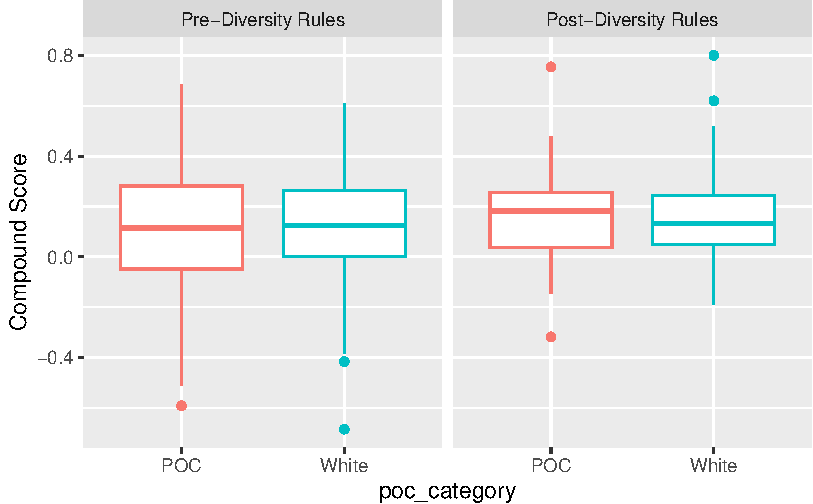
\includegraphics{Survivor_files/figure-pdf/Data-Cleaning-1.pdf}

}

\caption{Average Compound Scores of 184 Players from Survivor, Pre- and
Post- Implementation of Diversity Casting Rules}

\end{figure}

\hypertarget{operational-validity-of-first-confessionals}{%
\subsection{Operational Validity of First
Confessionals}\label{operational-validity-of-first-confessionals}}

We used a player's first confessional which matched the criteria
outlined in Figure I, which attempts to isolate confessionals relating
to personal strategy, motivations, and relationships, to capture the
first impression that viewers receive of the attitude of a player,
which, regardless of the player's overall season story arc, acts as a
foundation with which the viewers contextualize the rest of the player's
game.

\begin{Shaded}
\begin{Highlighting}[]
\NormalTok{knitr}\SpecialCharTok{::}\FunctionTok{include\_graphics}\NormalTok{(}\StringTok{"Flowchart.jpeg"}\NormalTok{)}
\end{Highlighting}
\end{Shaded}

\begin{figure}[H]

{\centering 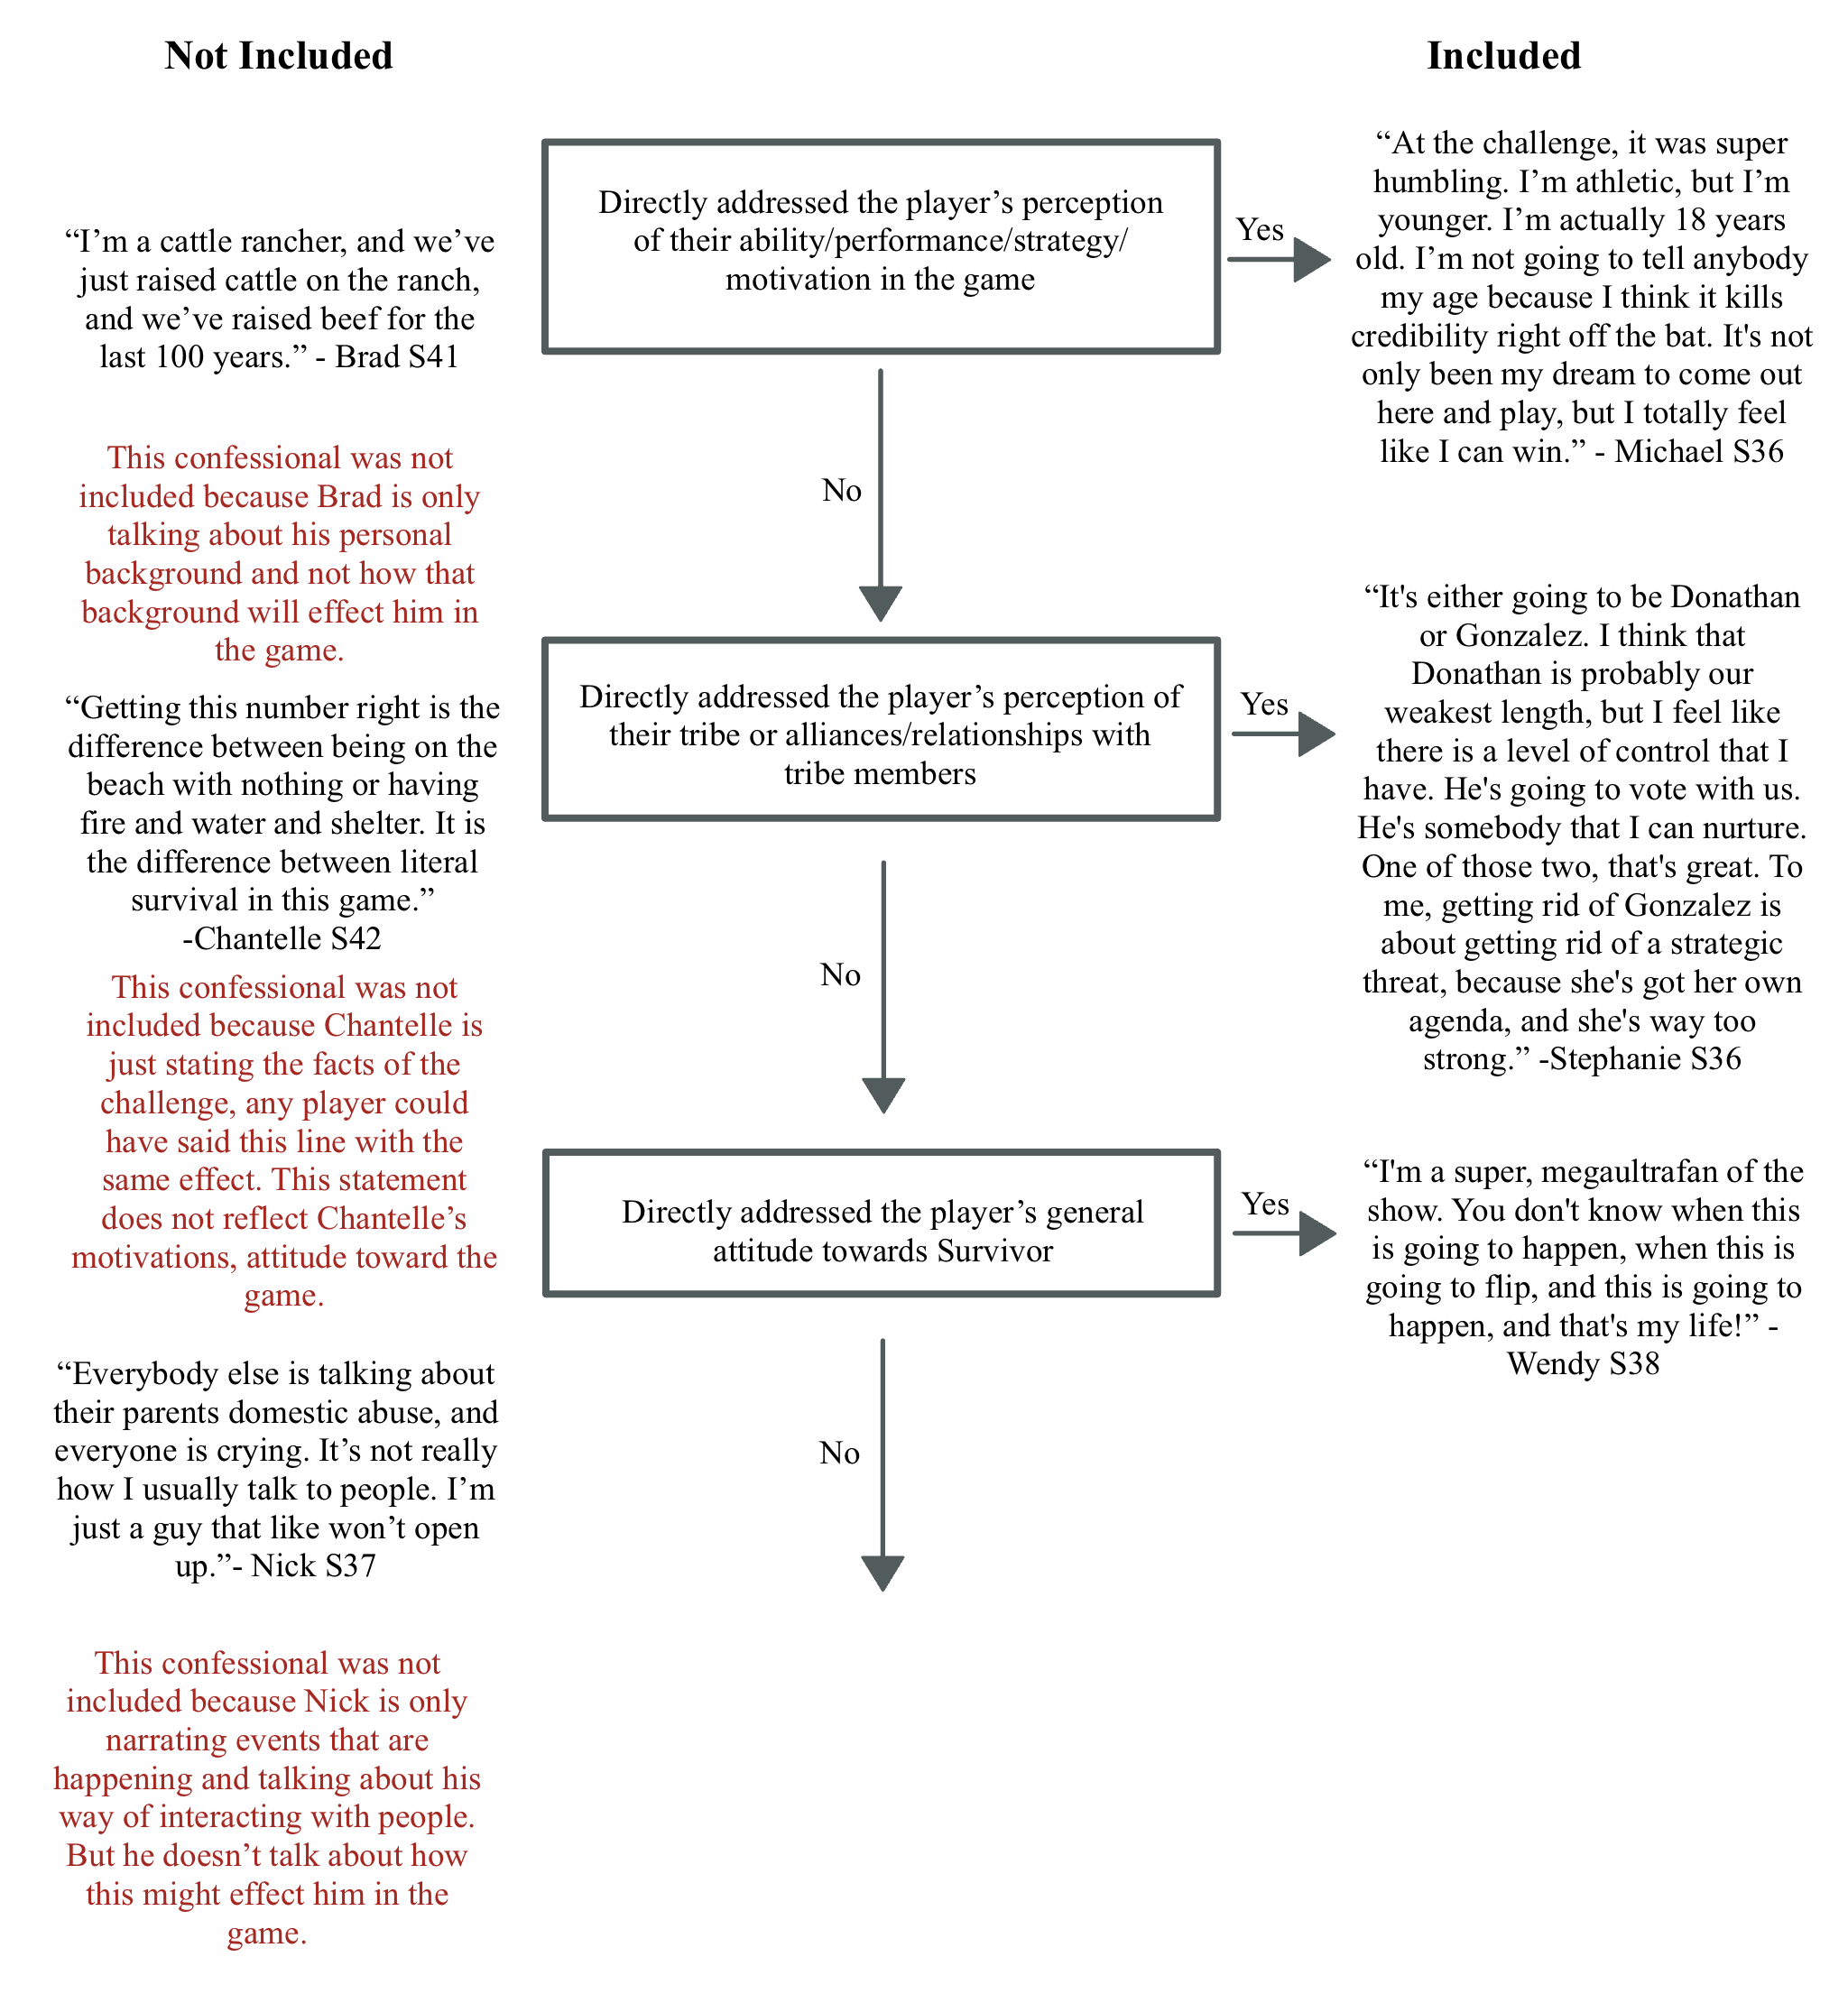
\includegraphics[width=4.6875in,height=\textheight]{Flowchart.jpeg}

}

\caption{Confessional Selection Diagram}

\end{figure}

Four players lacked confessionals which met the guidelines outlined in
Figure and were coded as negative by default, as our team took a lack of
portrayal as having a negative impact on a player's portrayal.

\hypertarget{dataset}{%
\subsection{Dataset}\label{dataset}}

The combined dataset includes information on the gender, age, race,
name, and POC status of each player in addition to their confessional,
sentiment analysis score, and portrayed initial attitude.
Figure~\ref{fig-3} is a visual representation of the portrayed attitudes
of poc and non-POC players pre- and post- diversity rules. Visually, the
stacked bar plots show an increase in the percentage of POC players in
the casts post-diversity rules as expected. Of these POC players, the
proportion whose initial, portrayed attitudes were analyzed as positive
seems to have increased compared to before the diversity casting rules
were implemented. However, this increase in positive portrayal also
appears with white players post- diversity casting rules as well. This
suggests the rough idea that perhaps, the diversity rules may have had
no or a very small effect on the nature in which POC players' initial
attitudes were portrayed, although this difference, or lack thereof,
will be explored more formally in our statistical analysis.

\begin{verbatim}
Warning: The dot-dot notation (`..count..`) was deprecated in ggplot2 3.4.0.
i Please use `after_stat(count)` instead.
\end{verbatim}

\begin{figure}

{\centering 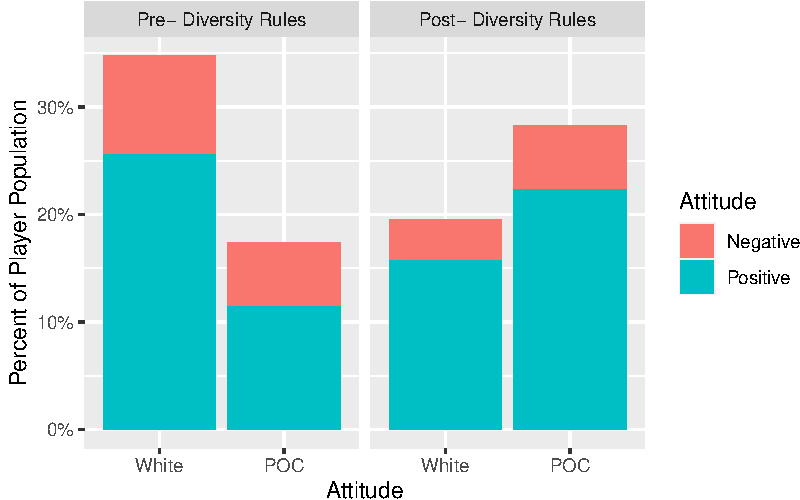
\includegraphics{Survivor_files/figure-pdf/fig-3-1.pdf}

}

\caption{\label{fig-3}Positive and Negative Portrayed Attitudes of 184
Players from Survivor, Pre- and Post- Implementation of Diversity
Casting Rules}

\end{figure}

\hypertarget{statistical-analysis-and-model}{%
\subsection{Statistical Analysis and
Model}\label{statistical-analysis-and-model}}

Using multiple logistic regression, our study will fit a model to the
dataset to investigate the existence of a relationship between the
log-likelihood of a portrayed positive initial attitude towards the game
with the player's status as a person of color, before the implementation
of diversity casting rules (Seasons 36-40) and after the implementation
of diversity casting rules (Seasons 41-45). Our study also will
investigate whether this relationship is moderated by the accounting of
other key factors of season of appearance, age, and gender. Selection of
the demographic factors for our model is based upon the sizable interest
and proclaimed importance to success in both the physical and social
aspects of gameplay in the Survivor cultural sphere, as well as
limitations on data availability and study timeline.

The empirical model used to examine the determinants of a player's
initial, portrayed attitude is specified as:

\(logit \{P(Attitude_i=1|POC_i,Div\_Rules_i,Age_i,Gender_i,Season_i)\} = \beta_0 + \beta_1POC_i + \beta_2Div\_Rules_i + \beta_3Age_i+ \beta_4Gender_i + \beta_{5-13}Season_i + \beta_{14}POC_i*Div\_Rules_i\)

\begin{equation} Gender_i = \begin{cases} 1 & \text{ if } i \text{ person identifies as a man} \\ 0 & \text{ if } i \text{ person identifies as a woman} \end{cases} \end{equation}

where \texttt{POC} indicates whether a player is a person of color,
\texttt{Age} gives a player's age in years with 18 subtracted to account
for the minimum age for players, \texttt{Gender} indicates whether a
player is male or female, \texttt{Div\_Rules} indicates the
implementation of diversity casting rules on a season, \texttt{Season}
gives the season number (seasons 37-44, with season 36 and season 45
left out due to singularities), and an interaction term to account for
how the presence of the diversity casting rules affected the
relationship between a player's POC status and their log odds of a
positive, initial portrayed attitude.

We hypothesize that after the implementation of diversity casting rules,
the likelihood that a POC player had a positive portrayed initial
attitude towards the game meaningfully increased, even after accounting
for the age and gender of a player.

\hypertarget{results}{%
\section{Results}\label{results}}

We find that for players of the same age and gender playing on the same
season pre-diversity rule implementation, the predicted odds of a
player's first significant confessional portraying a positive attitude
are 34.6\% lower for players of color than white players
(\(95\% \text{ CI}: 76.6\% \text{ lower}, 66.1\% \text{ higher}\)). For
players of the same age and gender playing on the same season
post-diversity rule implementation, the predicted odds of a player's
first significant confessional portraying a positive attitude are 11.3\%
lower for players of color than white players
(\(95\% \text{C I}: 70.4\% \text{ lower}, 166\% \text{ higher}\)).
Comparing seasons pre- and post-diversity rule implementation, we find
that the predicted odds ratio for POC versus White players becomes
smaller after the diversity rules are implemented, suggesting that the
diversity rules have a positive association with the odds that a player
of color has a positive, initially portrayed attitude in their first
significant confessional.

The results of our logistic regression are tabulated in
Table~\ref{tbl-regression-output}.

\hypertarget{tbl-regression-output}{}
\begin{table}
\caption{\label{tbl-regression-output}Regression Output of Model Considering Player POC Status, Age, Gender,
Season, and Diversity Rules Effect on Log Odds of Initial, Portrayed
Attitude of Player }\tabularnewline

\centering
\begin{tabular}{l|r|r|r|r}
\hline
  & Estimate & Std. Error & z-Statistic & P-Value\\
\hline
Intercept & 0.53 & 0.57 & 0.93 & 0.35\\
\hline
POC & -0.47 & 0.50 & -0.95 & 0.34\\
\hline
Div\_Rules & 1.40 & 0.95 & 1.46 & 0.14\\
\hline
Age & 0.01 & 0.02 & 0.26 & 0.79\\
\hline
Gender & 0.32 & 0.36 & 0.90 & 0.37\\
\hline
Season 37 & 1.21 & 0.81 & 1.50 & 0.13\\
\hline
Season 38 & -0.18 & 0.69 & -0.26 & 0.80\\
\hline
Season 39 & 0.30 & 0.71 & 0.42 & 0.67\\
\hline
Season 40 & 0.29 & 0.74 & 0.39 & 0.70\\
\hline
Season 41 & -1.50 & 0.91 & -1.65 & 0.10\\
\hline
Season 42 & -0.84 & 0.94 & -0.89 & 0.37\\
\hline
Season 43 & -0.82 & 0.94 & -0.87 & 0.39\\
\hline
Season 44 & -0.05 & 1.06 & -0.04 & 0.96\\
\hline
POC:Div\_Rules & 0.35 & 0.75 & 0.47 & 0.64\\
\hline
\end{tabular}
\end{table}

All of the individual coefficients have p-values greater than the 95\%
confidence threshold of \(p=0.05\). For our predictors of interest in
relation to our initial hypotheses--the POC status of the player, the
implementation of the diversity rules, as well as a player's age and
gender--, this result indicates that none of these predictors when
considered together along with our other predictors controlling for
potential season editing clusters were associated with changes in the
log odds of an initial, portrayed positive attitude for a player.

Supporting the results of our Wald tests on the individual coefficients,
we also find using a likelihood ratio test that the overall model is not
significant (\(p=0.58\)), and that an intercept-only model is sufficient
to predict the log odds of an initial positive portrayed attitude of a
player. Comparing preliminary models without age and gender predictors
to our full model for this analysis, we also found that the addition of
these two predictors was insignificant (\(p = 0.6304\)) in meaningfully
improving model fit to the data. Consequently, age and gender are also
insignificant as individual predictors in our final model
(\(p = 0.7924; p = 0.3657\)). See the Appendix for full results of
regression analyses for the reduced models utilizing the age and gender
predictors.

\emph{add table that shows odds ratios which are much more interpretable
than the log odds table that we have}

\hypertarget{discussion}{%
\section{Discussion}\label{discussion}}

Following the cultural reckoning caused by the broad social movement
associated with the George Floyd Protests of 2020, many workplaces and
businesses responded by implementing diversity, equity, and inclusion
(DEI) initiatives. Evaluating the efficacy of these DEI initiatives is
an important task and challenge for organizations as they seek to
improve workplace equity in the future.

Previous research has shown the importance of diverse racial
representation in fiction-based media on people's identity development
https://www.ncbi.nlm.nih.gov/pmc/articles/PMC4900900/, response to
advertising, and . The present study extends upon this work by
attempting to discern the effects of diverse racial representation on
the portrayal of reality competition show players of color from a media
consumer perspective.

In concurrence with the findings of related literature of the positive
effects of DEI initiatives on people of color in workplace contexts
(https://www.emerald.com/insight/content/doi/10.1108/17554211111162471/full/html),
our study found that after the diversity casting rules were implemented,
the difference in difference of the odds of a player of color having an
initial positive, portrayed attitude compared to a white player had
decreased. This decrease in the difference in odds suggests that
increasing the percentage of players of color on a season of Survivor
was associated with an increased likelihood that a player of color would
be initially, positively portrayed.

This association may be due to a variety of interacting components, such
as a change in editing and storyarc strategies or a change in mindset of
the players of color themselves. This association may also have
implications for how Survivor studio efforts to increase Survivor
viewership, as previous studies have shown that people tend to seek out
media at increased rates which strengthen their in-group identification
and the positivity they associate with it
(https://www.communications.k-state.edu/doc/marketing-research/age-identification-social-identity-gratifications-and-television-viewing.pdf).

Our study's finding of the positive association between age and the odds
of a player having an initial positive, portrayed attitude disagrees
with some researchers who have found negative relationships between age
and job well-being (https://www.jstor.org/stable/24720284?seq=10). Our
study's finding of the positive association between being male and the
odds of a player having an initial positive, portrayed attitude also
disagrees with many researchers who, to their surprise, have found no
differences in overall, or even increased job satisfaction in women
compared to men. Discerning the mechanisms which drive job satisfaction,
as well as many other work-related items, is ongoing. Our study speaks
to the mechanisms at play in reality competition shows, which likely
meaningfully differ from those relevant in the typical workplace due to
the idiosyncratic performance demands and social dynamics in a specific
reality competition show environment.

\hypertarget{limitations-and-further-research}{%
\section{Limitations and Further
Research}\label{limitations-and-further-research}}

Accurate regression analyses relies on, first and foremost, accurate
data with which to fit a model to. Primary-source data-gathering from
the CBS network as well as the players themselves, as opposed to
collaborative, second-hand citizen-science efforts which constructed our
study's dataset, in the future will be crucial to evaluating the effect
of diversity casting rules on the initial portrayals of the players of
color of Survivor.

Our investigation also may have benefitted from a larger sample size;
our present samples were limited to 17-20 players with significant
confessionals for each of the 10 seasons included. As additional seasons
of Survivor with diversity casting rules in place are produced, the
scope of future research models may expand to include additional seasons
before and after the updated casting rules took effect. Our study also
chose to exclude the singular nonbinary player due to lack of data on
those of their gender. A larger sample size may also introduce a
sufficient number of nonbinary players such that this population could
be represented in analyses. Overall, additional observations will
increase the statistical power of our study, decreasing the error
associated with our model predictors which increases the chance we
detect the effect of the casting rules if it exists, perhaps yielding
significant model predictors, which we did not have in our study.

Additionally, there may be more valid methods to evaluate the portrayed
attitude of a player. Confessionals alone may not be fully indicative of
a players' portrayed attitudes, as conversations with other players
often capture attitude as well. Our team's use of the VADER sentiment
analyzer to construct the attitudes of the confessionals in our dataset
may also pose limitations as this tool itself relies on a model,
introducing error into the process of polarity classification for
confessionals. Alternative methods of sentiment analysis using recurrent
neural networks or machine learning algorithms may be more accurate at
capturing the true sentiment of player confessionals to measure player
portrayal. Even better at measuring the player portrayal would be
sufficiently large, randomly-sampled viewer surveys about the perception
of the different players, which could be aggregated and averaged to
generate a numerical summary of how each player's initial attitude was
portrayed.

Logistic regression analysis may not be best-suited for analyzing our
dataset. As can be explored further in the Appendix, all assumptions of
regression were not met despite various transformations to the relevant
variables (notably \texttt{Age}), indicating more advanced regression
techniques may be appropriate for future research.

\hypertarget{conclusion}{%
\section{Conclusion}\label{conclusion}}

Overall, we consider our study to be a preliminary investigation into
one aspect in the holistic assessment of the efficacy of CBS' diversity
casting rules in Survivor. Our study found a positive association
between the implementation of diversity casting rules on the odds that a
player of color would have an initial, positive portrayed attitude, even
after accounting for the player's age and gender. Crucial to note, our
study did not find that this association was significant; thus, while
our findings do not rule out the existence of an effect of the diversity
casting rules on the odds that a player of color would have an initial,
positive portrayed attitude, it does not confirm that one exists,
either. We emphasize that our study be taken as preliminary, and highly
recommend that further research on this matter be conducted on this
facet and well as other facets of the diversity casting rules using
sufficiently large sample-sizes, primary source data, and sufficient
context-specificity as per our aforementioned recommendations before
conclusions are made as to the efficacy CBS' diversity casting rules on
players of color' initial portrayals and other relevant metrics.

\hypertarget{appendix}{%
\section{Appendix}\label{appendix}}

\hypertarget{summary-stats}{%
\section{Summary Stats}\label{summary-stats}}

\hypertarget{demographics}{%
\subsection{Demographics}\label{demographics}}

\hypertarget{tbl-summary-stats}{}
\begin{table}
\caption{\label{tbl-summary-stats}Demographic Characteristics of the Players in the Study Population }\tabularnewline

\centering
\begin{tabular}[t]{l|l}
\hline
\cellcolor{black}{\textcolor{white}{\textbf{Characteristic}}} & \cellcolor{black}{\textcolor{white}{\textbf{Value}}}\\
\hline
\textbf{Gender} & \textbf{}\\
\hline
Male - no. (\%) & 91 (49.46)\\
\hline
Female - no. (\%) & 93 (50.54)\\
\hline
\textbf{Age - yr.*} & \textbf{}\\
\hline
All & 32.80 ± 8.95\\
\hline
\textbf{Race - no (\%)**} & \textbf{}\\
\hline
Asian/Pacific Islander & 28 (15.22)\\
\hline
Black & 39 (21.11)\\
\hline
Hispanic or Latino & 17 (9.24)\\
\hline
White & 100 (54.35)\\
\hline
\textbf{Season - no. (\%)} & \textbf{}\\
\hline
36 & 20 (10.87)\\
\hline
37 & 20 (10.87)\\
\hline
38 & 18 (9.78)\\
\hline
39 & 20 (10.87)\\
\hline
40 & 18 (9.78)\\
\hline
41 & 17 (9.24)\\
\hline
42 & 18 (9.78)\\
\hline
43 & 18 (9.78)\\
\hline
44 & 17 (9.24)\\
\hline
45 & 18 (9.78)\\
\hline
\multicolumn{2}{l}{\rule{0pt}{1em}\textit{Note: }}\\
\multicolumn{2}{l}{\rule{0pt}{1em}* Mean age of players ± Std. Deviation, ** Race as provided by the Survivor Wiki}\\
\end{tabular}
\end{table}

\hypertarget{assumptions}{%
\section{Assumptions}\label{assumptions}}

Multiple logistic regression relies on the assumptions that the response
is a Bernoulli random variable, observations are independent, and the
predictors show a linear relationship with the log odds of the response.
Our response is a Bernoulli random variable because it takes one of two
values- 1 indicating a positive portrayed attitude and 0 indicating a
negative portrayed attitude. Our selection criteria for player
confessionals lead to independence as players do not interact while
making these statements, and player demographics are inherently
independent.

Among our predictors, gender, POC status, season, and presence of
diversity casting rules are all binary, automatically satisfying the
linearity assumption.

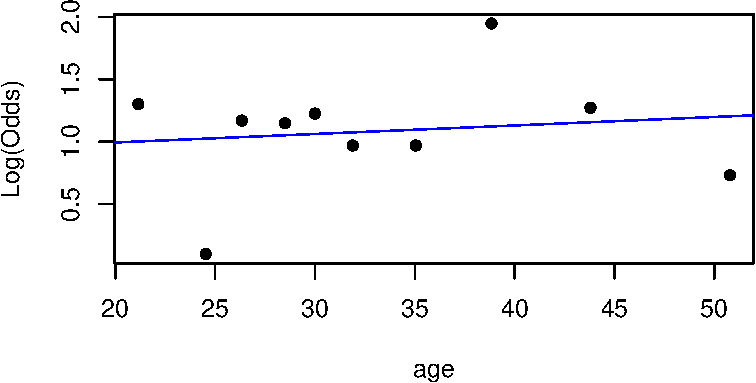
\includegraphics{Survivor_files/figure-pdf/label-3-1.pdf}

However, an empirical logit plot of our only numerical predictor, age,
shows violation of the linearity assumption as the estimated log odds
follow a curved trend against age. This violation persisted after
exploring several transformations of the age variable, thus we chose not
to transform the variable to maintain interpretability.

\hypertarget{model-selection}{%
\section{Model Selection}\label{model-selection}}

To assess the significance of our model, we conducted a likelihood ratio
test under the hypotheses
\[H_0: logit \{P(Attitude_i=1|POC_i,Div\_Rules_i,Age_i,Gender_i,Season_i)\} = \beta_0\]

\[H_A: logit \{P(Attitude_i=1|POC_i,Div\_Rules_i,Age_i,Gender_i,Season_i)\} = \beta_0 + \beta_1POC_i + \]
\[\beta_2Div\_Rules_i + \beta_3Age_i+ \beta_4Gender_i + \beta_{5-13}Season_i + \beta_{14}POC_i*Div\_Rules_i\]

\hypertarget{tbl-full-anova}{}
\begin{table*}

\begin{table}
\caption{\label{tbl-full-anova}Likelihood Ratio Test Results for Full Model }\tabularnewline

\centering
\begin{tabular}{l|r|r|r|r|r}
\hline
Model & Resid. DF & Resid. Deviance & DF & Deviance & P-Value\\
\hline
Attitude \textasciitilde{} 1 & 183 & 206.94 & NA & NA & NA\\
\hline
Attitude \textasciitilde{} poc * div\_rules + age\_adj + gender + season & 170 & 195.57 & 13 & 11.37 & 0.58\\
\hline
\end{tabular}
\end{table}

\end{table*}

To assess the significance of age and gender in our model, we conducted
a second likelihood ratio test under the hypotheses

\[H_0: logit \{P(Attitude_i=1|POC_i,Div\_Rules_i,Age_i,Gender_i,Season_i)\} = \beta_0 + \beta_1POC_i + \]
\[\beta_2Div\_Rules_i + \beta_{5-13}Season_i + \beta_{14}POC_i*Div\_Rules_i\]

\[H_A: logit \{P(Attitude_i=1|POC_i,Div\_Rules_i,Age_i,Gender_i,Season_i)\} = \beta_0 + \beta_1POC_i + \]
\[\beta_2Div\_Rules_i + \beta_3Age_i+ \beta_4Gender_i + \beta_{5-13}Season_i + \beta_{14}POC_i*Div\_Rules_i\]

\hypertarget{tbl-reduced-anova}{}
\begin{table*}

\begin{table}
\caption{\label{tbl-reduced-anova}Likelihood Ratio Test Results for Reduced Model }\tabularnewline

\centering
\begin{tabular}{l|r|r|r|r|r}
\hline
Model & Resid. DF & Resid. Deviance & DF & Deviance & P-Value\\
\hline
Attitude \textasciitilde{} poc * div\_rules + season & 172 & 196.50 & NA & NA & NA\\
\hline
Attitude \textasciitilde{} poc * div\_rules + age\_adj + gender + season & 170 & 195.57 & 2 & 0.92 & 0.63\\
\hline
\end{tabular}
\end{table}

\end{table*}



\end{document}
